
%%%%%%%%%%%%%%%%%%%%%%%%%%%%%%%%%%%%%%%%%%%%%%%%%%
\chapter{Production Optimization}
%%%%%%%%%%%%%%%%%%%%%%%%%%%%%%%%%%%%%%%%%%%%%%%%%%
The optimization of oil production is a tedious and computational intensive 
process that requires the solution of time dependent nonlinear set of partial 
differential equations describing the flow of hydrocarbons in anisotropic porous 
media. The optimization of time-varying well settings, such as injection rates, 
production rates or bottom-hole pressures, is an important aspect of optimal 
reservoir management. Optimization of production is usually performed using either gradient 
free techniques like genetic, particle swarm algorithms, or gradient-based 
techniques where the gradients are computed through the solution of the adjoint 
problem.

\section{Gradient-free methods}
In this section we review the basic gradient-free method
employed in industry and academia for the solution of several
optimal control problems of the oil industry.
\subsection{Genetic algorithms (GAS)}
Genetic algorithms are commonly used to generate high-quality solutions to 
optimization and search problems by relying on bio-inspired operators such as 
mutation, crossover and selection.The method is a general one, capable of being 
applied to an extremely wide range 
of problems.
Genetic algorithms are based on three essential components:

- Survival of the fittest (Selection).

- Reproduction processes where genetic traits are propagated (Crossover).

- Variation (Mutation).
\subsection{Particle Swarm Optimization(PSO)}
Particle swarm optimization (PSO) is  is a stochastic, population-based computer algorithm.
It applies the concept of swarm intelligence (SI) to problem solving.
Swarm intelligence is the property of a system whereby the collective behaviors of 
(unsophisticated) agents interacting locally with their environment cause 
coherent functional global patterns to emerge (e.g. self-organization, emergent 
behavior). Gradient-free methods are not necessarily guaranteed to find the true global 
optimal solutions, but they are able to find many good solutions.

\section{Gradient-based methods}
Gradient-based optimization methods offer the advantage to construct additional 
information about the shape of the surface for the particular problem. Hence, 
the gradient of a function provides information about the behavior of a 
function such as steepness and extrema in the parameter space. The gradients are 
computed through the solution of the adjoint problem.  With this additional 
information, the convergence of the search algorithm can be drastically 
enhanced.
\subsection{Sequential quadratic programming (SQP) }
Sequential quadratic programming (SQP) is an iterative procedure that utilizes a 2.order approximation of
the Lagrangian function of a problem. The quadratic formulation of the problem is a local approximation
of the real problem and consists of a quadratic objective function and linear equality
and/or inequality constraints. SQP can be used both within a trust-region and a line
search framework. In a line search framework, the algorithm proceeds by first calculating
a search direction. If we are trying to maximize the original problem, a function is then
solved that maximize the quadratic approximation in the search direction. When a
new iteration point in the direction that was searched has been reached, a new local
approximation is constructed and the algorithm proceeds to the next iteration given that
a set of optimality conditions has not been fulfilled.
SQP is a generalization of Newtons method for unconstrained problems as it uses a
quadratic approximation of the Lagrangian function, steps in a direction it believes the
optimum lies, and then creates a new approximation of the original model when a new
iteration point has been reached. The main difference between Newtons method and
SQP is that for constrained nonlinear problems the Taylor approximation of the original
problem cannot be used, as the model problem also needs to incorporate the constraints
of the original problem. Instead, the Lagrangian function is used and the constraints of
the problem thereby taken into account. SQP is appropriate for small and large problems and it 
is well-suited to solving problems with significant nonlinearities\citep{Bonnans}.
\subsection{Interior point optimization (IPO)}
An interior point method is a linear or nonlinear programming method that 
achieves optimization by going through the middle of the solid defined by the 
problem rather than around its surface. This method is further discussed in section....


Both gradient-based and derivative-free methods have been considered for this 
problem, and both are applicable in different situations. 
A gradient-based optimization method, in which the gradient is computed using 
an adjoint formulation, is often the method of choice since in contrast to 
numerical perturbation techniques that require as many objective function 
evaluations as the number of control parameters, the gradient using 
adjoint-based techniques is obtained  only at a small fraction of the time 
spent for the evaluation of the objective function.  The development of adjoint 
procedures for general compositional flow problems is 
much more challenging than black-oil simulation because of the need to perform
phase-equilibrium (flash) calculations for all grid blocks at every iteration 
of every time step. Adjoint formulations are challenging to code
because they require analytical derivatives of many variables, and the
increased complexity of compositional simulators renders these derivatives
much more cumbersome to calculate than in the case of a black-oil simulator.
Furthermore, the production optimisation problem is usually subject to industrial 
constraints, for example, maximum gas rate specification in injection or 
production wells, when the control variables are well bottom-hole pressures. At 
the same time optimising  time-varying well settings, such as injection rates, 
production rates or bottom-hole pressures, is an important aspect of optimal 
reservoir management that increases significantly the dimension of the search 
space. It is well known that for non-convex optimisation problems, 
gradient-based techniques are likely get trapped in poor local optima. A common 
practise is to lunch several independent optimisation from different initial 
guesses or to combine ideas from gradient-free algorithms with gradient-based 
to benefits from the merits of both. An adequate sampling of the search space 
would require an intractable number of simulations and it is thus impossible.



%%%%%%%%%%%%%%%%%%%%%%%%%%%%%%%%%%%%%%%%%%%%%


\section{Oil-gas compositional simulation equations} \label{sec:forward}


The mass conservation equation for component $i$, which can exist in any
phase $j$ (here $j=o,~g$, where $o$ indicates oil and $g$ gas), is given
by \cite{Cao:Thesis,Voskov_nonlinear:2009,Voskov:2012}:
%
\begin{align}
\label{transport_eq_ci}
\dfrac{\partial}{\partial t} \left(\phi
  \sum_{j} x_{ij} \rho_j S_j \right)
    - \nabla \cdot \left ( \sum_{j} x_{ij} \rho_j  \boldsymbol{\tens{K}}
      \dfrac{k_{rj}}{\mu_j}\nabla \Phi_j \right ) + \\ \sum_{w} \sum_{j} x_{ij} \rho_j q_j^w = 0, \ \ i = 1,\ldots,n_c. \nonumber
\end{align}
%

In the first (accumulation) term, $t$ is time, $\phi$ is porosity, $x_{ij}$
designates the mole fraction of component $i$ in phase $j$, $S_j$ is saturation,
and $\rho_j$ is molar density. In the second (flow) term,  $\boldsymbol{\tens{K}}$ 
is the permeability tensor, $k_{rj}$ is the relative permeability to
phase $j$, $\mu_j$ the phase viscosity, and the phase potential
$\Phi_j$ is given by $\Phi_j = p_j-\rho_j g(D-D^0)$, where $p_j$ is
phase pressure, $D$ is depth, $D^0$ is a reference depth, and $g$ is
gravitational acceleration. In the third (source/sink) term, $q_j^w$
indicates the phase flow rate for well $w$. The treatment of this term will be discussed in Section~\ref{sec:constr-sim}. Equation~(\ref{transport_eq_ci}) is written for each of the $n_c$
components present in the system.

For a mixture of $n_c$ components in two fluid phases (oil and gas), thermodynamic equilibrium
can be expressed as:
%
\begin{equation} \label{general_therm_system1} f_{io}(p_o, x_{io}) - f_{ig}(p_g,
  x_{ig}) = 0,  \end{equation}
%
where $f_{io}(p_o, x_{io})$ is the fugacity of component $i$ in the oil phase and $f_{ig}(p_g, x_{ig})$ 
is the fugacity of component $i$ in the gas phase (temperature does not appear because the system is assumed to
be isothermal).
%and $n_p$ is the number of phases (here $n_p=2$).
We additionally must satisfy the saturation constraint ($S_o+S_g=1$) and the
component mole fraction constraints:
%
\begin{align}\label{eqn:MoleFractionCons} \sum_{i=1}^{n_c} x_{i0} -1 = 0, \ \ \
    \ \ \ \ \sum_{i=1}^{n_c} x_{ig} -1 = 0.  \end{align}
%
A capillary pressure relationship also appears in cases with nonzero capillary
pressure, though here we neglect capillary pressure so $p_o=p_g$.

As discussed by many authors (see, e.g.,
\cite{Coats:1980,Cao:Thesis,Voskov:2012,Young:1983}), the system described
above contains a total of only $n_c$ primary equations and primary variables per
grid block. These equations and variables are coupled (from block to block), and
in a fully-implicit method are all computed simultaneously at each Newton
iteration. The remaining (secondary) variables can be computed locally (block by
block), and thus very efficiently, once the primary variables are determined.
Various options exist for the choice of primary variables (see
\cite{Voskov:2012} for discussion). Here we use the so-called natural variable
set, which includes, for each grid block, one pressure unknown, $n_p-1$
saturation unknowns (where $n_p$ is the number of phases; here $n_p=2$), and $n_c-n_p$ component mole fraction unknowns.

In our formulation, the governing equations (\ref{transport_eq_ci}) are solved
fully-implicitly, using a backward-Euler time discretization, two-point flux
approximation, and single-point upwinding \cite{Aziz_book79}. These treatments
are standard in practical reservoir simulation. For the solution of the set of
nonlinear equations, we use Newton's method with the solution at the previous
time step as the initial guess. A limit on the change of the grid-block
saturation and mole fractions over a Newton iteration is applied
\cite{Younis:2010}. The Newton iterations terminate when the maximum relative
norm of the residual is less than $10^{-6}$ (tight convergence criteria are required for the adjoint solution, discussed below). For the solution of the
linear system at each Newton iteration we use GMRES preconditioned by the
constrained pressure residual method, as described in~\cite{CPRA}. Iteration is
terminated when the Euclidean norm of the initial residual has decreased by five
orders of magnitude.

We employ a simple time stepping strategy. The time step size at step $n+1$ is a
multiple of that at $n$, provided nonlinear convergence was achieved at step
$n$. In this way the time step can increase until it reaches the maximum
allowable value. If the nonlinear solver fails to converge within a prescribed number
of Newton iterations, we divide the time step by a fixed constant. This process
is repeated until the nonlinear system converges.



\section{Adjoint equations for the compositional system} \label{sec:adjoint}
We now present the discrete and continuous adjoint equations. Some numerical and coding issues are also discussed.


\subsection{Automatic differentiation} \label{sec:autodiff}


It is quite common for comprehensive computational platforms, in reservoir
simulation and other application areas, to undergo frequent modification and enhancement. This poses a problem for adjoint formulations
because, when an existing feature is modified the corresponding adjoint code may
also be impacted, and when a new feature is added, the associated adjoint code
must (in many cases) be written. The maintenance and development of adjoint code
poses challenges because the necessary derivatives are generally complicated.
This is particularly the case in compositional simulation where variables couple
in many ways, including through the nonlinear equation of state.


Automatic differentiation, or AD, is gaining popularity in the field of
scientific computing as a means of facilitating the development and enhancement of large code bases. AD enables, for example, the fast (analytical) determination of Jacobian matrix elements from the code
defining the residual vector. The use of AD has allowed the fast construction
and assessment of different compositional formulations within the same code
\cite{Voskov_nonlinear:2009}. In this work, we take advantage of AD to automate
the construction of many of the derivatives required for the adjoint
formulation.


The AD implementation used in our compositional simulator is the `automatic
differentiation expression templates library' (ADETL), developed originally by
Younis and Aziz~\cite{Younis:2007}.  This library generates efficient computer
code for the evaluation of the Jacobian matrix and the corresponding partial
derivatives from discrete algebraic expressions of the governing conservation
equations, associated constraint relations, and equations of state. We refer to
\cite{Younis:2007} for a detailed description of the underlying theory.


\subsection{Discrete adjoint formulation} \label{section:discreteAdjoint}

Following the fully-implicit discretization of the governing equations (using the usual finite volume method, with treatments as noted above), we can express the nonlinear system as:
%
\begin{align}
\label{eq:DiscretizedEquations}
\p_n(\x_n, \x_{n-1}, \u_n) =  \0 \rm,
\end{align}
%
where $\p_n$ denotes the fully discretized, both in space and time,
set of partial differential equations. Here $\x_n = \x(t_n)$ and $\u_n =
\u(t_n)$ are the states and controls (well settings), respectively, at time step $n$. The corresponding time step size
is designated $\Delta t_n$. We will use throughout the notation $\partial \p^T / \partial \x$ to denote the matrix $(\partial \p / \partial \x)^T$.



We are interested in either maximizing or minimizing
an objective function $\myobj$ that is in general a nonlinear function of the
states $\x_n$ and the controls $\u_n$ of the forward problem. We
assume that $\myobj$ has the following form:
%
\begin{align}
  \label{eq:continuousObjective}
  \myobj(\x, \u) = \integral{\F\left ( \x(t), \u(t) \right )} + \M(\x(t_N)),
\end{align}
%
where $\F(\x(t), \u(t))$ is a nonlinear function varying with time and $\M(\x(t_N))$ is a
function of only the last state $\x_N$. After the solution of the
forward problem has been obtained, $\myobj$ may be approximated by
%
\begin{align}
  \label{eq:discretizedObjective}
  \myobj \approx \fsum{n=1}{N}{ \Delta t_n \, \F_n \left ( \x_n, \u_n \right ) + \M(\x_N) }.
\end{align}
%

Using (\ref{eq:discretizedObjective}) we can state the optimal control
problem as:
%\\
%\begin{tabular}{ll}
%Extremize  &
%  $\displaystyle f =
%  \fsum{n=1}{N}{ \Delta t_n \, \F_n \left ( \x_n, \u_n \right ) + \M(\x_N) }$ \\
%  subject to &
%$\p_n(\x_n, \x_{n-1}, \u_n) = \0$, \\
%and &
%$\x_0 = \x(t_0)$.
%\end{tabular}
%\\ \\
\[
   \newproblem{NLP}{\u}{\displaystyle \myobj =
  \sum_{n=1}^N \Delta t_n \, \F_n \left ( \x_n, \u_n \right ) + \M(\x_N) }
                 {\p_n(\x_n, \x_{n-1}, \u_n) = \0,}
                 {\x_0 = \x(t_0)}.
\]

In general, a number of linear and nonlinear constraints may need to be included in the optimal
control problem. We postpone the discussion of their treatment until Section~\ref{sec:constraints}. 
Now, since $\p_n = \0$, we can introduce the augmented objective function $\myobj_A$ by `adjoining' 
the governing equations to the original objective function $\myobj$. The new objective $\myobj_A$ shares
the same extrema as $\myobj$ and is defined as:
%
\begin{align}
\label{eq:JAdefinition}
  \myobj_A = \fsum{n=1}{N}{\left ( \Delta t_n \F_n(\x_n, \u_n)
      + \blambda^T_n \p_n (\x_n, \x_{n-1}, \u_n)  \right )}
   + \M(\x_N).
\end{align}
%
In (\ref{eq:JAdefinition}), the vectors $\blambda_n$ are the Lagrange multipliers.


The maximum or minimum of $\myobj_A$ (and thus $\myobj$) is achieved when the first variation of $\myobj_A$ is 
zero ($\delta \myobj_A=0$). After performing some index-shifting, and grouping
terms multiplied by the same variation ($\delta \x_n, \delta \x_N,
\delta \u_n$), $\delta \myobj_A$ can be written as:
%
\begin{align}
\label{eq:discreteAfterRegrouping}
  \delta \myobj_A &=
  \left (
    \pder{\M_N}{\x_N}
    + \Delta t_N \pder{\F_N}{\x_N}
    + \blambda_N^T\pder{\p_N}{\x_N}
    \right ) \delta \x_N
    \nonumber \\
    &+\fsum{n=1}{N-1}{
      \left (
        \Delta t_n \pder{ \F_n}{\x_n}
        +\blambda^T_{n+1}\pder{\p_{n+1}}{\x_n}
        +\blambda^T_n\pder{\p_n}{\x_n}
      \right ) \, \delta \x_n
    } \nonumber \\
    &+\fsum{n=1}{N}{
      \left (
        \Delta t_n \pder{\F_n}{\u_n}
        +\blambda^T_n\pder{\p_n}{\u_n}
      \right ) \, \delta \u_n.
    }
\end{align}
%
In order to achieve $\delta \myobj_A=0$, we require $\delta \myobj_A / \delta \x_n=\0^T$ (for $n=1,2, \ldots, N$) and $\delta \myobj_A / \delta \u_n=\0^T$. To satisfy $\delta \myobj_A / \delta \x_n =\0^T$ for $n=1,2, \ldots, N$, we require that the Lagrange multipliers satisfy the following equations:
%
\begin{align}
\label{eq:discreteODE}
 \pder{\p_n^T}{\x_n}  \blambda_n &= -
 \left (\pder{\p_{n+1}^T}{\x_n} \blambda_{n+1} + \Delta t_n \pder{\F^T_n}{\x_n}
 \right ),% \quad n=1,2,\ldots,N-1
\\
\label{eq:discreteBC}
  \pder{\p_N^T}{\x_N} \blambda_N &= -
  \left ( \Delta t_N \pder{\F^T_N}{\x_N} + \pder{\M_N^T}{\x_N} \right ).
\end{align}
%
With this choice of the Lagrange multipliers the total variation becomes
\begin{align*}
  \delta \myobj_A =
    \fsum{n=1}{N}{
      \left (
        \Delta t_n \pder{\F_n}{\u_n}
      +\blambda^T_n\pder{\p_n}{\u_n}
      \right ) \, \delta \u_n ,
    }
\end{align*}
and the gradient of the objective function with respect to the controls is
\begin{align}
\label{eq:optimizerDiscreteGradient}
  \frac{\delta \myobj_A}{\delta \u} = \left [
  \frac{\delta f_1}{\delta \u_1}, \frac{\delta f_2}{\delta \u_2},
  \ldots,
  \frac{\delta f_N}{\delta \u_N} \right ].
\end{align}
The individual entries of $\delta \myobj_A/\delta \u$ are given by
%\footnote{If possible give some proof of this derivation}
\begin{align}
\label{eq:discreteGradient}
  \frac{\delta f_n}{\delta \u_n} =
  \Delta t_n  \pder{\F_n}{\u_n}
  +\blambda^T_n\pder{\p_n}{\u_n}, \quad n=1,2,\ldots,N.
\end{align}
%
By driving $\delta \myobj_A / \delta \u$ to zero, we achieve the minimum or 
maximum of $\myobj_A$ (and thus $\myobj$). In practice, $\delta \myobj_A / \delta \u$, 
along with other quantities related to constraints, are provided to a 
gradient-based optimization algorithm to determine the next estimate for the controls $\u$.

In optimization problems, the well control variables do not typically change at each time step in the flow simulation. Rather, they are defined over longer time periods that are referred to as control steps. Time steps are usually small in order to capture flow dynamics, reduce time-discretization error, and facilitate convergence of the Newton iterations. 
The gradient at the control period $m$, $\delta f_n/\delta \u_m$, is simply the sum of
the gradients $\delta f_n/\delta \u_n$ for all time steps that belong to control period $m$.


\subsection{Continuous adjoint formulation}
\label{section:continuousAdjoint}
The continuous adjoint formulation employs the continuous
representation of the objective function along with the spatially discretized reservoir flow equations. The optimal control problem can then be stated as:
%\\
%\begin{tabular}{ll}
%Extremize&
%  $\displaystyle f(\x, \u) = \integral{ \F(\x(t), \u(t)) } + \\M(\x(t_N))$
%\\
%subject to &
%$\p(\dot{\x}(t), \x(t), \u(t) ) = \0$.
%\end{tabular}
%\\ \\
\[
   \problem{}{\u}{\displaystyle \myobj(\x, \u) = \integral{ \F(\x(t), \u(t)) } + \M(\x(t_N))}
                 {\p(\dot\x(t), \x(t), \u(t) ) = \0.}
\]


In this case we express the governing set of partial differential
equations, for a specified dynamic well-control strategy $\u(t)$, as $\p(\dot{\x}(t), \x(t), \u(t) ) = \0$.  
We introduce the Lagrange multipliers $\blambda(t)$  and define the Lagrangian $\L$ as:
%
\begin{align}
  \label{eq:lagrangian}
  \L(\dot{\x}, \x, \u, \blambda) = \F(\x, \u) + \blambda^T \, \p(\dot{\x}, \x, \u ),
\end{align}
%
The
variables $\u(t)$, $\x(t)$, $\dot{\x}(t)$ and $\blambda(t)$ are denoted
as $\u$, $\x$, $\dot{\x}$ and $\blambda$ to simplify notation. The
augmented objective function, $\myobj_A$, can be expressed as:
%
\begin{align}
  \myobj_A(\dot{\x}, \x, \u, \blambda) = \integral{\L(\dot{\x}, \x, \u, \blambda)} + \M(\x_N).
\end{align}
%
The first variation of $\myobj_A$ is given by
%
\begin{align}
\label{eq:firstvariation}
  \delta \myobj_A
  &= \integral{
    \left (
    \pder{\L}{\dot{\x}} \, \delta \dot{\x}
  + \pder{\L}{\x} \, \delta \x
  + \pder{\L}{\u} \, \delta \u
  + \pder{\L}{\blambda} \, \delta \blambda \right ) }
  \nonumber \\
  &+ \pder{\M(\x_N)}{\x_N} \, \delta \x_N.
\end{align}
%
Note that $\delta \dot{\x} = d (\delta \x) / d t$, so any variation in
the state vector $\x$ will introduce a
variation in its time derivative $\dot{\x}$.

After integration by parts, using the fact that the variation of the initial conditions $\delta \x_0 = \0$, and
taking into account that $\partial \L^T / \partial \blambda = \p(\dot \x, \x, \u) \, = \0$,
the first variation of $\myobj_A$ can be written as:
%
\begin{align}
\label{eq:augmentedobjective}
  \delta \myobj_A
  &= \integral{
    \left(
      \pder{\L}{\x}  -\dder{}{t} \pder{\L}{\dot{\x} }
    \right) \, \delta \x} \nonumber \\
 &+ \left ( \pder{\L(\x_N)}{\dot{\x}_N} + \pder{\M(\x_N)}{\x_N} \right )
  \, \delta \x_N \nonumber \\
  &+ \integral{ \pder{\L}{\u} \, \delta \u }.
\end{align}
%
To achieve $\delta \myobj_A / \delta \x=\0$, $\blambda$ must be chosen
to satisfy the following:
%
\begin{align}
\label{eq:continuousadjointode}
  &\dder{}{t} \left ( \pder{ \p^T }{\dot \x} \blambda \right )
    - \pder{\p^T}{\x} \blambda - \pder{\F^T}{\x} = \0
\\
\label{eq:terminatingbc}
&\pder{\p^T_N}{\dot{\x}_N} \blambda_N = -\pder{\M^T(\x_N)}{\x_N}.
\end{align}
%
The ordinary differential equation in (\ref{eq:continuousadjointode}) is integrated backwards in
time starting from the final time condition
(\ref{eq:terminatingbc}). With the resulting $\blambda$, the first variation of the objective function becomes:
\begin{align}
  \delta \myobj_A = \integral{ \left ( \pder{\F}{\u} + \blambda^T
      \pder{\p}{\u} \right ) \, \delta \u}.
\end{align}


In order to allow a direct comparison of the discrete and continuous adjoint formulations,
we integrate the continuous adjoint backwards in time fully implicitly,
using the same scheme as is applied for the forward problem. The discrete
form of (\ref{eq:continuousadjointode}) is:
\begin{align}
  \label{eq:continuousODE}
  \pder{\p^T_n}{\x_n} \blambda_n
  = -  \pder{\p^T_{n+1}}{\x_n} \blambda_{n+1} -
   \Delta t_n \pder{\F^T_n}{\x_n}.
\end{align}
This equation is solved backwards in time, starting from the boundary condition~(\ref{eq:terminatingbc}).
Once the Lagrange multipliers have been obtained, the gradient is computed using
equations~(\ref{eq:optimizerDiscreteGradient}) and (\ref{eq:discreteGradient}). 
 

\subsection{Continuous versus discrete adjoint formulation}
The gradients obtained by the discrete adjoint formulation are, as would be
expected, fully consistent with the discrete forward problem. Indeed, if we
compute the gradients using numerical perturbation of the controls, we find that
they coincide with those from the discrete adjoint solution in the first 5-8
significant digits (to achieve this level of agreement, tight tolerances must be
used for linear and nonlinear convergence of the forward simulation). There are differences, however,
between these gradients and those provided by the continuous adjoint
formulation.

To illustrate this, consider
the simplified case where $\M(\x_N) = 0$. The solution of
(\ref{eq:terminatingbc}) in this case will give $\blambda_N = \0$,
and as a result, the first term in (\ref{eq:discreteAfterRegrouping})
will not vanish. There will be a nonzero term left multiplying the
variation of $\delta \x_N$:
%
\begin{align}
\label{eq:discreteAfterRegroupingWithContinuousBC}
  \delta \myobj_A &=
  \Delta t_N \pder{\F_N}{\x_N} \delta \x_N
  +\fsum{n=1}{N}{
      \left (
        \Delta t_n \pder{\F_n}{\u_n}
        +\blambda^T_n\pder{\p_n}{\u_n}
      \right ) \, \delta \u_n.
    }
\end{align}
It is evident that, as the time step size $\Delta t_N \rightarrow 0$,
the term multiplying $\delta \x_N$ will vanish, and the gradient provided by the continuous
formulation will become consistent with that from the discrete problem.
However, as long as $\Delta t_N$ is significant, the two gradients
will not coincide, especially at the last time step.



We implemented both the continuous and discrete adjoint formulations into our
optimization framework. Using a small $\Delta t_N$, we observed that the
computed gradients were very similar, consistent with
(\ref{eq:discreteAfterRegroupingWithContinuousBC}). Even using small $\Delta
t_N$, however, we did not observe any advantage of the continuous formulation
over the discrete formulation. In cases where $\Delta t_N$ was not small, the
continuous formulation required more iterations of the optimizer, presumably
because of errors in $\delta \myobj_A / \delta \u$. In light of these observations,
we do not present any detailed results using the continuous adjoint
formulation since we do not see any advantages to this approach for our
problem. We note that these finding are consistent with those reported
in~\cite{Hager2000} and \cite{Walther2007} for general Runge-Kutta
time stepping methods, 
in~\cite{Nadarajah:2000}, where the discrete and continuous adjoint
approaches were applied to automatic  aerodynamic optimization, and
in~\cite{Petra2011} for general variational inverse problems governed
by partial differential equations. A
 similar gradient discrepancy between discretization/optimization
 versus optimization/discretization can also occur with respect to the
 spatial discretization -- see the discussion for a shape
 optimization problem in~\cite{GunzburgerBook}. 



\subsection{Solution of adjoint equations} The solution of the linear system of
equations that arises when solving (\ref{eq:discreteODE}) constitutes the
largest computational demand in the adjoint problem. The matrix appearing in
this equation at time step $n$, $\partial {\p_n^T}/\partial {\x_n}$, is
the transpose of the Jacobian matrix for the converged forward problem,
    $\partial {\p_n}/\partial {\x_n}$. In our implementation, the converged
    states are written to disk during the solution of the forward problem. These
converged states are then read back, during the solution of the adjoint problem,
          and $\partial {\p_n}/\partial {\x_n}$ is reconstructed, along with all
other derivatives appearing in equations (\ref{eq:discreteODE}),
      (\ref{eq:discreteBC}) and (\ref{eq:discreteGradient}). This enables the
      evaluation of the Lagrange multipliers $\blambda_n$ and the gradients
      $\partial f_n/\partial {\u_n}$.


For the solution of the linear system in (\ref{eq:discreteODE}), we use
GMRES preconditioned by the transpose of the CPR (constrained
pressure residual) preconditioner, as described in~\cite{CPRA}. In these
linear solutions, we require very high accuracy to guarantee that residual
errors accumulated over hundreds of time steps do not pollute the gradients
(which would influence the computed optimum). For this reason, we continue
iterating the linear solver until the Euclidean norm of the initial residual has
decreased by 10 orders of magnitude. This is significantly higher accuracy than
is required for the forward problem.




\section{Gradient-based optimization and related software}
\label{sec:SQPSNOPT}

The \SNOPT{} optimizer is used in this work for solving the nonlinear constrained
optimization problem, and in this section we will provide a concise overview of the underlying theory. This discussion loosely follows \cite{SNOPT}, which provides a much more in-depth description. We note that the adjoint formulation described in this paper may also be used in conjunction with other optimization packages. \SNOPT{} uses a sparse sequential quadratic
programming (SQP) algorithm that exploits sparsity in
the constraint Jacobian and maintains a limited-memory quasi-Newton
approximation to the Hessian of the Lagrangian. The QP
subproblems are solved using an inertia-controlling reduced-Hessian
active-set method (\SQOPT) that allows for variables appearing
linearly in the objective and constraint functions. 
 
%\subsection{The SQP approach}


%%%%%%%%%%%%%%%%%%%%%%%%%%%%%

% \subsection{Notation}  \label{sec-notation}
%
%Some important quantities follow:
%$$
%\begin{tabular}{ll}
%        $(\u, \blambda, \s)$               & primal, dual and slack variables,
%\\[2pt] $(\xstar, \blambdastar, \sstar)$ & optimal variables,
%\\[2pt] $(\u_k, \blambda_k, \s_k)$         & the $k$th estimate of $(\ustar,\blambdastar,\sstar)$,
%\\[2pt] $f_k$, $\g_k$, $\c_k$, $f_k$  & functions and gradients evaluated at $\u_k$,
%\\[2pt] $(\uhat_k,\blambdahat_k,\shat_k)$& optimal variables for QP subproblem (\GQPk).
%\end{tabular}
%$$

 %%%%%%%%%%%%%%%%%%%%%%%%%%%

We now discuss the main features of the SQP method used to solve our
nonlinear program (NP). This discussion follows~\cite{SNOPT}. As will be discussed in detail in Section~\ref{sec:constr-opt}, all realistic recovery optimization problems involve bound constraints on the inputs, and often several other linear or nonlinear equality or inequality constraints, which together constitute a so-called general nonlinear program (GNP). All features described in this section are readily specialized to the GNP discussed in Section~\ref{sec:constr-opt}. Here we take the problem to be
$$
   \problem{(NP)}{\u}{f(\u)}{\c(\u) \ge 0,}
$$
where $\u \in \mathbb R^n$, $\c \in \mathbb R^m$, while the objective function $f(\u)$ and the constraints $c_i(\u), \; i=1,2,\ldots,m$
have continuous second derivatives. The gradient of $f$ is denoted
by the vector 
$\grad f(\u)$, 
%$\g(\u)$
and the gradients of each element of $\c$ form
the rows of the Jacobian matrix $\J(\u)$.

An SQP method obtains search directions (for the primal $\u$ and dual variables $\bpi$) from an iterative sequence of QP subproblems. Each QP subproblem, in turn, iteratively minimizes a convex quadratic
model of a certain Lagrangian function subject to
linearized constraints associated with (NP), namely,
\begin{equation}                                 \label{eqn-def-ML}
        \Lscr(\u,\u_k,\bpi_k) = f(\u) - \bpi_k^T \dL(\u,\u_k),
\end{equation}
defined in terms of the constraint linearization $\cL(\u,\u_k)$
and the departure from linearity $\dL(\u,\u_k)$:
\begin{eqnarray*}
        \cL(\u,\u_k) &=& \ck  + \Jk(\u - \u_k),
     \\ \dL(\u,\u_k) &=& \c(\u) - \cL(\u,\u_k),
\end{eqnarray*}
subject to linearized constraints. In this formulation $k$ is the SQP (major) iteration counter, and $\bpi$ are Lagrangian multipliers to adjoin $\dL$ to $f$. The first and second derivatives of the modified Lagrangian with
respect to $\u$ are
\begin{eqnarray*}
        \grad\Lscr(\u,\u_k,\bpi_k) &=& \grad f(\u) - (\J(\u) - \Jk)\T \bpi_k, \\[3pt]
        \Hess\Lscr(\u,\u_k,\bpi_k) &=& \disp \Hess f(\u)
                                           - \sum_i (\bpi_k)_i \Hess c_i(\u).
\end{eqnarray*}
Observe that $\Hess\Lscr$ is independent of $\u_k$
and is the same as the Hessian of the conventional Lagrangian.
At $\u = \u_k$, i.e., after convergence of the inner iterations, the modified Lagrangian has the same function and
gradient values as the objective:
$
           \Lscr(\u_k,\u_k,\bpi_k) = \fk, \ %\qquad
     \grad \Lscr(\u_k,\u_k,\bpi_k) = \grad \fk.
$
The modified augmented Lagrangian is `less' nonlinear than the augmented Lagrangian itself
because linear terms in the constraints disappear, especially in the quadratic penalty term.
The number of nonlinear variables in the modified augmented Lagrangian is the same as in the original problem.

The merit function 
\begin{equation}                              \label{eqn-def-merit}
        \Mscr_\rho(\u,\bpi,\s)
          = f(\u) - \bpi\T \bigl( \c(\u) - \s \bigr)
            + \half \sum_{i=1}^m \rho_i\big( c_i(\u) - s_i\big)^2,
\end{equation}
where $\rho$ and $\s$ are vectors of penalty parameters and slack variables, respectively, 
is reduced along each search
direction to ensure convergence from any starting point.

In summary, the basic structure of an SQP method involves major and
minor iterations.  The major iterations generate a sequence of
iterates $(\u_k,\bpi_k)$ that converge to the optimal solution $(\ustar,\bpistar)$.
At each major iterate a QP subproblem is solved to generate a search direction
towards the next iterate $(\u\kp1,\bpi\kp1)$.
Solving such a subproblem is itself an iterative procedure, and the minor iterations of an
SQP method are the iterations of the QP method.
\SNOPT{} requires first-order derivatives of the nonlinear
objective and constraint functions with respect to the control variables, which
are provided by our adjoint procedure.



\section{Nonlinear constraints} \label{sec:constraints} 
Several authors have discussed the incorporation of constraints in the optimal
control problem for oil recovery optimization. This includes partial and 
sometimes heuristic approaches, valid for particular types of constraints 
\cite{Brouwer:2004,VanEssen,Virnovski,Wang:2009}, and more systematic 
approaches, valid for a broader range of constraint equations 
\cite{Chen:2010,Montleau,Kraaijevanger,Pallav:2008,Suwartadi:2012}. An important 
feature in simulations involving highly compressible fluids, which we have in 
the systems considered here since we inject gas, is the occurrence of transient 
peaks in the rate in response to changes in well bottom-hole pressure 
(bottom-hole pressure, or BHP, is the wellbore pressure at a specified depth 
within the reservoir). These transient effects impact simulation results in our 
models because they occur over time scales that are larger than a time step 
(this is in contrast to nearly incompressible systems, where this type of 
transient decays very quickly and is not resolved by the simulator). These 
transient effects lead to challenges in constrained optimization of 
compositional systems, because rate constraints can be easily violated. Here we 
will present and assess both a formal constraint handling approach and a simpler 
heuristic procedure for satisfying rate constraints, which can be used in 
compressible systems.
% 
% Many constraints appear as simple bound constraints (e.g., bottom hole 
% pressure (BHP) limits in a problem where BHPs are the control variables), 
% but in other cases the constraints are nonlinear since a (nonlinear) simulation 
% is required to evaluate them. An example of this is the specification of maximum 
% gas production rate (either for an individual well or for a group of wells) in a 
% general compositional problem where the control variables are BHPs. In this 
% section we discuss the handling of nonlinear constraints. We describe a detailed 
% treatment within the optimizer, and an approximate heuristic treatment in the forward model.



\subsection{Constraint handling in the optimizer} \label{sec:constr-opt}
In the presence of nonlinear output inequality constraints, 
it can be difficult to determine an initial guess for the control parameters 
that does 
not violate these constraints. In such cases
the optimizer must apply a process to find a feasible set of control parameters. 
Some optimizers may also intentionally exit the feasible region, in an attempt 
to (eventually) find better optima. For these reasons, constraint and 
infeasibility handling are key architectural components of any general purpose 
optimizer. Here we described how they are handled within \SNOPT{}. 

To simplify notation, we first write the constrained optimization problem in the 
more 
general form (GNP) assuming lower and upper bounds on the controls and the 
nonlinear
constraints
$$
   \problem{(GNP)}{\u \in \mathbb R^n}{f(\u)}
      {\b_l \le \pmat{\u\\\c(\u)\strutl} \le \b_u,}
%   \problem{(GNP)}{\u \in \mathbb R^n}{f(\u)}
%      {\b_l \le \pmat{\u\\\c(\u)\\\A\u \strutl} \le \b_u,}
$$
where $f(\u)$ is a linear or nonlinear objective function,
$\c(\u)$ is a vector of nonlinear constraint functions $c_i(\u)$
with sparse derivatives, and $\b_l$ and $\b_u$
are vectors of lower and upper bounds.
We assume that the nonlinear functions are smooth and that their first
derivatives are available.

\subsubsection{Achieving feasibility} \label{sec-infeas}

\SNOPT{} deals with infeasibility using $\ell_1$ penalty functions.
%First, infeasible linear constraints are detected by solving a problem
%of the form
%%
%%First, a conventional Phase 1 simplex algorithm is applied to the
%%linear constraints and bounds on $x$.  (This starts with any convenient
%%basis and minimizes the one-norm of infeasibilities for the
%%basic variables.)  If the linear constraints prove to be infeasible,
%%\SNOPT{} solves a problem of the form
%\[
%   \problem{}{\u,\v,\w}{\e^T(\v + \w)}{%
%                   \b_l \le \pmat{\u\\ \A\u - \v + \w \strutl} \le \b_u, \ \ %
%                   \v \ge 0,\ \ \w \ge 0,}
%\]
%where $\e$ is a vector of ones and $\v$ and $\w$ are handled implicitly.
%This is equivalent to minimizing the one-norm of the general linear
%constraint violations subject to the simple bounds---often called
%elastic programming in the linear programming literature
%\cite{BroG75b}. 
%  If the linear constraints are infeasible ($\v \ne 0$ or $\w \ne 0$),
%\SNOPT{} terminates without computing the nonlinear functions.
%Otherwise, all subsequent iterates satisfy the linear constraints.
%
%
It solves (GNP) as given, using QP subproblems
based on linearizations of the nonlinear constraints.
If a QP subproblem proves to be infeasible or unbounded (or if the
Lagrange multiplier estimates for the nonlinear constraints become
large), \SNOPT{} reverts to a technique known as `elastic programming' to solve the problem
\[
   \newproblem{(\GNP{\gamma})}{\u,\v,\w}{f(\u) + \gamma \, \e^T(\v + \w)}
                 { \b_l \le \pmat{\u\\ \c(\u) - \v + \w \strutl} \le \b_u,}
                 { \ \ \v \ge 0, \ \ \w \ge 0,}
%   \problem{(\NP{\gamma})}{\u,\v,\w}{f(\u) + \gamma \, \e^T(\v + \w)}
%                { \b_l \le \pmat{\u\\ \c(\u) - \v + \w \\\A\u \strutl} \le \b_u,
%                   \ \ \v \ge 0,\ \ \w \ge 0,}
\]
where $\e$ is a vector containing all ones and $\v$ and $\w$ are `elastic variables' which allow the constraints to stretch in directions that increase the size of the feasible region. The resistance to stretching is obtained by minimizing the composite objective function $f(\u) + \gamma \, \e^T(\v + \w)$, where the penalty parameter $\gamma$ ($\gamma \ge 0$) may take a
finite sequence of increasing values.  
If (GNP) has a feasible solution and $\gamma$ is sufficiently large,
the solutions to (GNP) and (\GNP{\gamma}) are identical.
If (GNP) has no feasible solution, (\GNP{\gamma}) will tend to
determine a `reasonable' infeasible point if $\gamma$ is again sufficiently
large.  If $\gamma$ were infinite, the nonlinear constraint violations would
be minimized subject to the linear constraints and bounds.

This process may require many major iterations until a feasible initial set of control parameters
is obtained. For this reason, optimization with simple bound constraints on 
the inputs usually converges much faster than optimization with additional bounds
on output quantities.

\subsubsection{Constraint lumping}

Many constraints appear as simple bound constraints (e.g., BHP limits in a problem where BHPs are the control variables), but in other cases the constraints are nonlinear since a (nonlinear) simulation is required to evaluate them. Examples of this are the specification of maximum 
gas injection or production rates (either for an individual well or for a group of wells) in a 
general compositional problem where the control variables are BHPs. A variety of methods have been proposed to incorporate nonlinear constraints in the adjoint formulation; see,
e.g.,~\cite{Pallav:2006,Jansen:2011,Suwartadi:2012,Chen:2010} for detailed discussion.
 
As indicated above, operational constraints in reservoir simulation are often inequality constraints specified for input and/or output rates at every time step. In some cases these constraints must be satisfied by many, or by all, of the wells in the problem.
This means that the vector $\c(\u)$ in (GNP) can be of dimension $O(N_w N)$, where $N$ is the number of time steps and $N_w$ is the number of wells. Computing the gradients
for each of the entries of $\c(\u)$, which is required by SNOPT, will require $N$ adjoint simulations and thus, in total, the solution of $O(N_w N^2)$ linear systems of equations in addition to each forward simulation. This may be
computationally intractable for realistically-sized problems.

A more efficient way of approximating these gradients 
is to `lump' the constraints over the full simulation time frame~\cite{Pallav:2008}. 
This lumping can be performed on a well-by-well basis, in which case $O(N_w N)$ linear systems 
must be solved for the evaluation of the gradient, or over the entire model, in which case only $O(N)$ linear systems must be solved. The approximate gradients of the lumped
nonlinear constraints are then obtained in the same manner as the gradient of the
objective function; i.e., in terms of time-step contributions. It is important to recognize that the approach used for constraint lumping can impact the performance of the optimization procedure. Bound constraints on the controls do not require any special treatment as they are readily handled by the optimizer.

Constraints that are described by nondifferentiable functions can be challenging
to incorporate. A constraint of this type that appears frequently in production
optimization problems is the maximum (or minimum) well flow rate constraint,
e.g.,
%
\begin{align}
q_{jn} \leq q_{max},
\end{align}
%
where $q_{jn}$ is the rate of the well $j$ at time step $n$ and $q_{max}$ is a specified maximum rate.
To satisfy this constraint we must guarantee that
\begin{align}
\max_{j,n}{(q_{jn})} \leq q_{max}.
\end{align}
However, the $\max$ function is not differentiable 
so it cannot be used to provide
gradient information.  We thus approximate it by a smooth
function, specifically one suggested by~\cite{Bertsekas}:
%
\begin{align} \label{eq:maxdef} &c = \max_{j,n}(q_{jn}) \approx \alpha
\log{Q}, \nonumber \\
&Q = \sum_{j=1}^{N_w}\sum_{n=1}^{N} e^{q_{jn}/\alpha}, \\ 
&\alpha = 0.05 q_{max}. \end{align}
%
With this definition of the constraint
function, the gradient of the constraint with respect to the control variables,
  which is required by the optimizer, is given by:
  %
\begin{align} \label{eq:constraintGradient} \frac{\delta c}{\delta \u_n} &=
\frac{1}{Q}\sum_{j=1}^{N_w} e^{q_{jn}/\alpha} \pder{q_{jn}}{\u_n} +\blambda^T_n\pder{\p_n}{\u_n},  
\nonumber \\
\pder{q_{jn}}{\u_{n}} &= \left [ 0, 0, \ldots, \pder{q_{jn}}{u_{jn}}, \ldots, 0 \right ].
\end{align}
%
The Lagrange multipliers for the constraints $\blambda_n$ are
computed from the solution of the following adjoint problem:
  \begin{align}
\label{eq:discreteODEConstraints}
 \pder{\p_n^T}{\x_n}  \blambda_n &= -
\pder{\p_{n+1}^T}{\x_n} \blambda_{n+1} + 
\frac{1}{Q}\sum_{j=1}^{N_w} e^{q_{jn}/\alpha} \pder{q^T_{jn}}{\x_n}, 
\\
\label{eq:discreteBCConstraints}
\pder{\p_N^T}{\x_N} \blambda_N &= -
\frac{1}{Q}\sum_{j=1}^{N_w} e^{q_{jN}/\alpha} \pder{q^T_{jN}}{\x_N}.
\end{align}
The smaller the coefficient multiplying $q_{max}$ in (\ref{eq:maxdef}), the more accurate the
approximation of $\max$ becomes. The numerical value used here, $0.05$, ensures
that no overflow occurs in any of the exponential terms in the summation. The
approximation of $\max$ in (\ref{eq:maxdef}) is always greater than the maximum
of the component well rates, so if this maximum is honored, the true constraint
is guaranteed to be satisfied.




\subsection{Constraint handling in the simulator}  \label{sec:constr-sim}

A simpler way to render an infeasible solution feasible, when the
constraints are upper and lower bounds on output quantities 
(e.g., rates when BHPs are specified), is to satisfy these constraints 
in the forward model. This is often readily accomplished because, during the forward
simulation, wells can be controlled by specifying either the bottom-hole 
pressure or the rate. In the former case,
the well rate $q_j^w$ for phase $j$ in block $l$ is calculated from the well model, which (subject to some simplifications) is of the general form
%
\begin{align}
\label{eq:wellrate}
  \left( q_j^w \right)_l = \left( T_w\frac{k_{rj}}{\mu_j} \right)_l (p_l - p_{w,l}),
\end{align}
%
where $T_w$ is the well index (or well transmissibility), $p_{w,l}$ is the 
wellbore pressure for the well in block $l$, and $p_l$ is the well-block pressure.
Here $p_{w,l}$ is related to the BHP through an additional well equation. 
%that also involves $q_j^w$.
When well rate is specified, equations of the form of (\ref{eq:wellrate}) 
can be used to compute $p_{w,l}$. For more details on well models, and on the 
relationship between $p_{w,l}$ and BHP, see \cite{Cao:Thesis}.
%


This flexibility in defining the controls of the wells allows some constraints
to be easily satisfied during the forward simulation. For example, if a maximum
gas production rate is specified and a well operating under BHP control violates
this maximum, the well can be switched from BHP control to rate control and
operated at the maximum rate. This treatment is illustrated in
Fig.~\ref{fig:BHPvsRateControl}. The BHP (top left) is prescribed to be 50~bar
throughout the simulation, but we also have a maximum gas rate of 5,000~m$^3/$d at reservoir conditions (indicated by the blue line in the upper right figure). The well operates at
50~bar for the first 480 days, at which point the maximum rate constraint is
reached. The well then switches to operate at a gas rate of 5,000~m$^3/$d for the
rest of the simulation. The resulting BHP and gas production rate profiles
actually used in the simulation (and which honor the constraints) are shown in
the bottom two figures.

In the results below, we apply this treatment and compare it to the formal approach described in Section~\ref{sec:constr-opt}. Using this procedure, which we refer to as `heuristic constraint handling', we first perform the optimization without including the nonlinear constraints. Bound (linear) constraints are honored during the optimization. Then, after this initial optimization has converged, we run the forward problem once more using the `optimized' BHPs, but this time the simulator is allowed to switch to rate control when required to satisfy the nonlinear constraints. Thus the computational effort for this approach is little more than that required for optimizing the bound (and linearly) constrained problem, as just one additional simulation run is performed.


In our implementation of the heuristic constraint handling procedure, we also allow wells to switch back to BHP control (after they have switched from BHP control to rate control). The switch in control is accomplished, in either case, by checking (at each Newton iteration) to see if the current active control is violated. This assessment can be performed efficiently through use of the well equation. If the well does switch back to BHP control, it remains on BHP control unless (and until) the rate constraint is again violated. This process generally increases the number of Newton iterations required for convergence, though in most of the cases considered the total simulation time is within a factor of two of that for a typical forward simulation run (and, as noted above, the run using heuristic constraint handling is only performed once). 


%Control
%switching from BHP to rate and vice versa takes place within each Newton
%iteration, whenever the rate constraint is violated for a specific well. The
%well equation ~\ref{eq:wellrate} provides an estimate of the corresponding
%well rate. If the estimated well rate exceeds the specified upper bound the
%simulator stops controlling the BHP and controls the rate, in order to enforce
%feasibility. The same well equation is used for estimating the BHP when the
%well is rate-controlled. As soon as the BHP is estimated to lie within the
%specified upper and lower bounds, the well switches back to BHP control and
%remains on BHP control until at some future time step the rate constraint is
%violated again.  This process usually increases the number of Newton
%iterations needed for convergence to the desired tolerance, but in most of the
%cases considered we never observed the simulation time increasing further than
%two times the simulation times needed for the unconstrained simulation. So
%overall our Heuristic approach will always be as efficient as the unconstrained
%optimization plus the extra time needed for this additional forward simulation
%where control switching takes place to enforce feasibility.



\begin{figure}[ht]
\begin{center}
  \begin{tabular}{cc}
    BHP control & Rate \\
    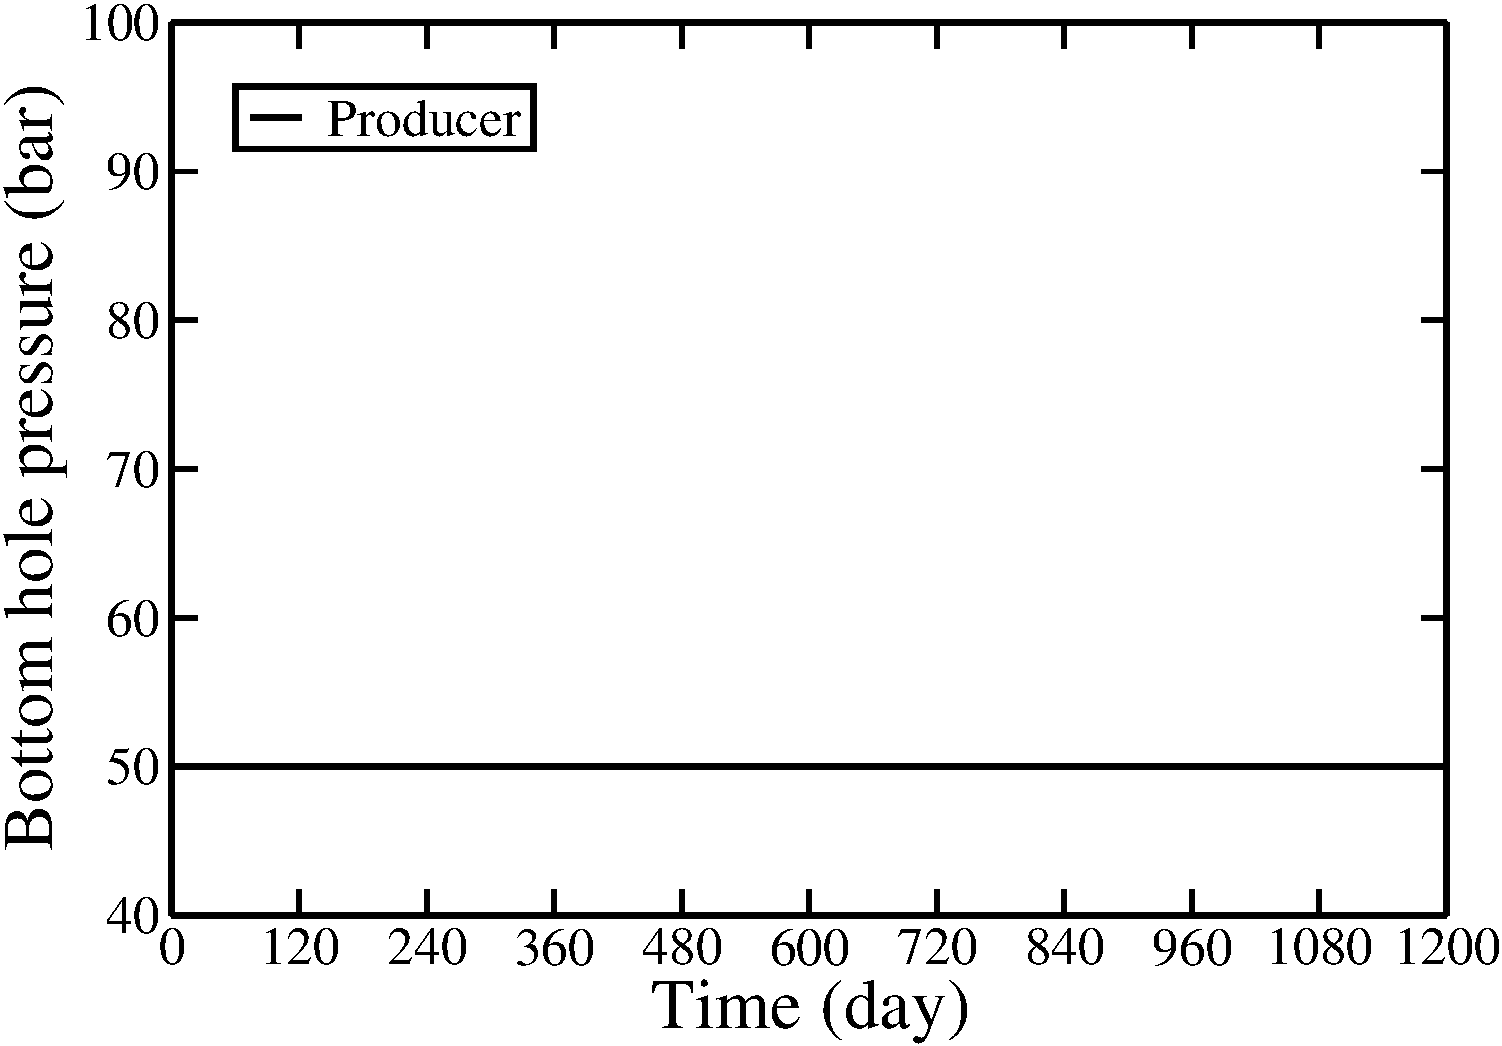
\includegraphics[height=2.7cm]{figures/SimpleBHP_BHP.pdf}
    &
    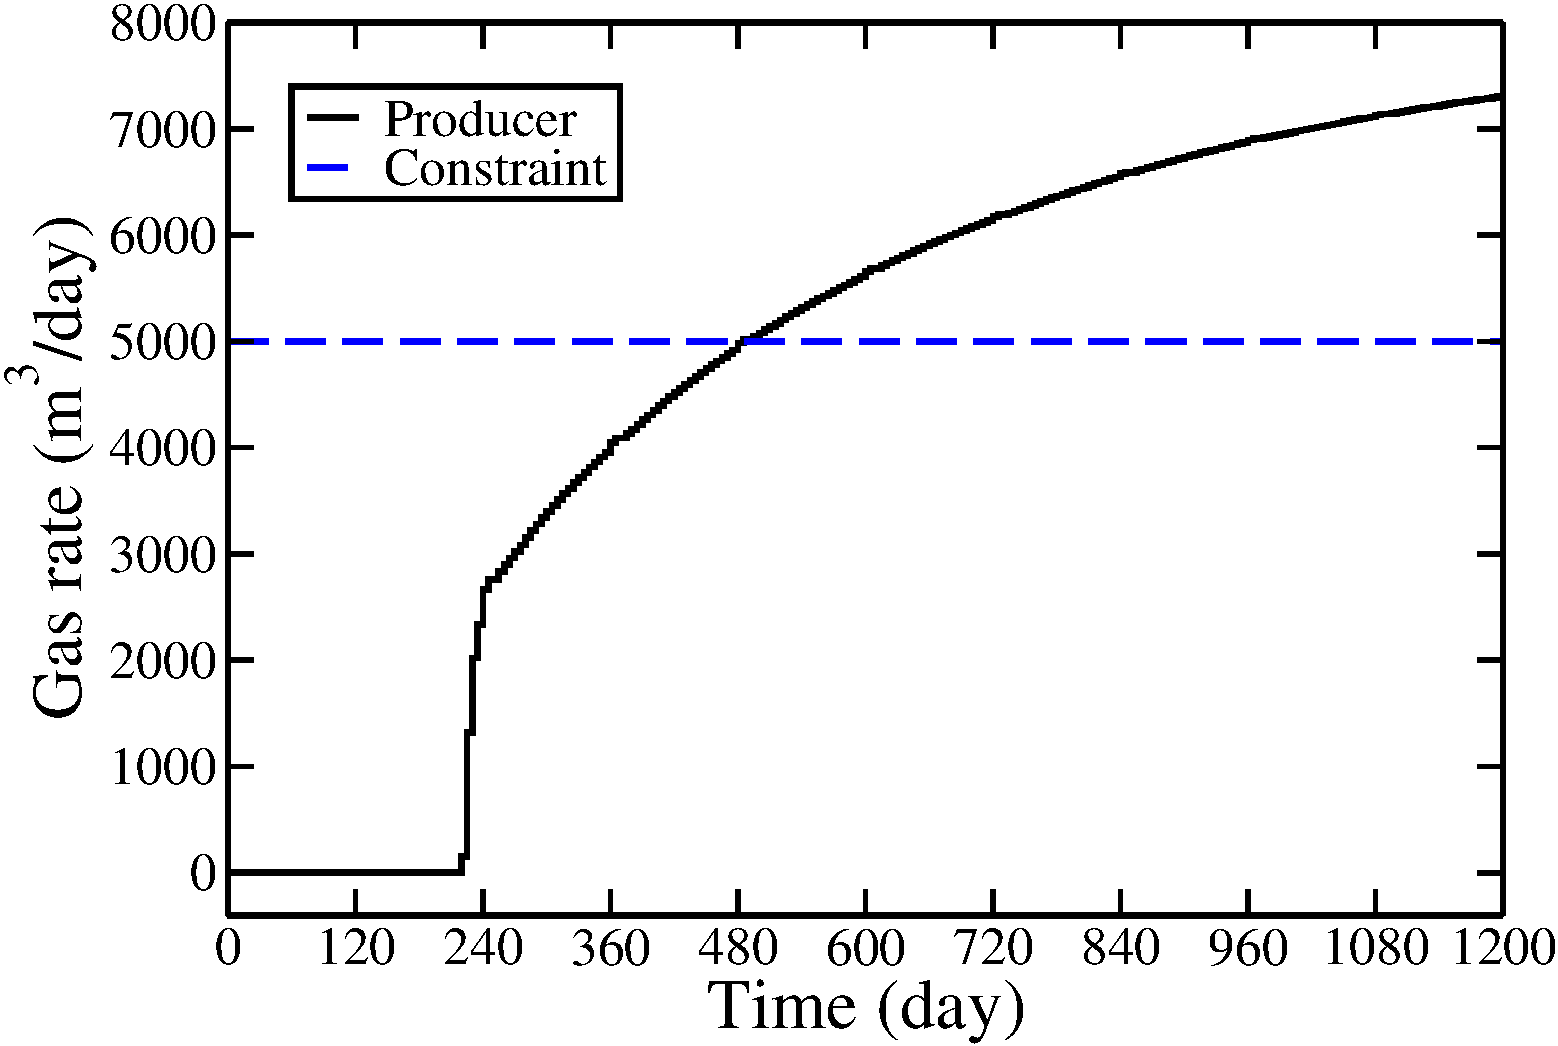
\includegraphics[height=2.7cm]{figures/SimpleBHP_rate_gas.pdf} \\
    BHP & Rate control \\
    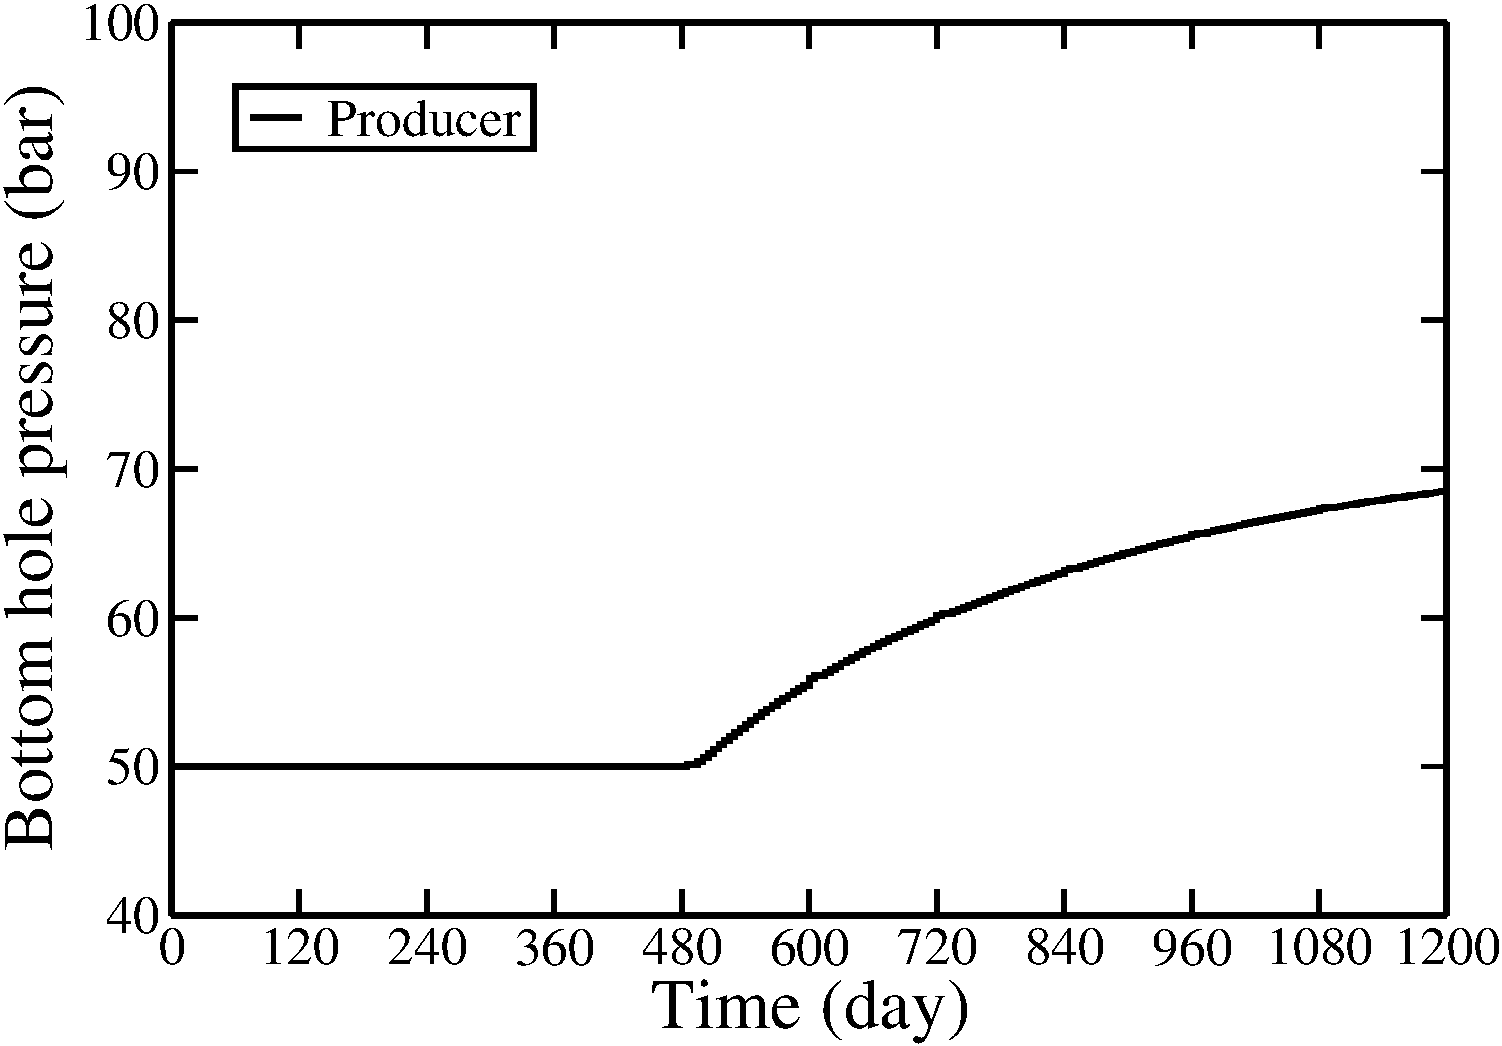
\includegraphics[height=2.7cm]{figures/SimpleRate_BHP.pdf}
    &
    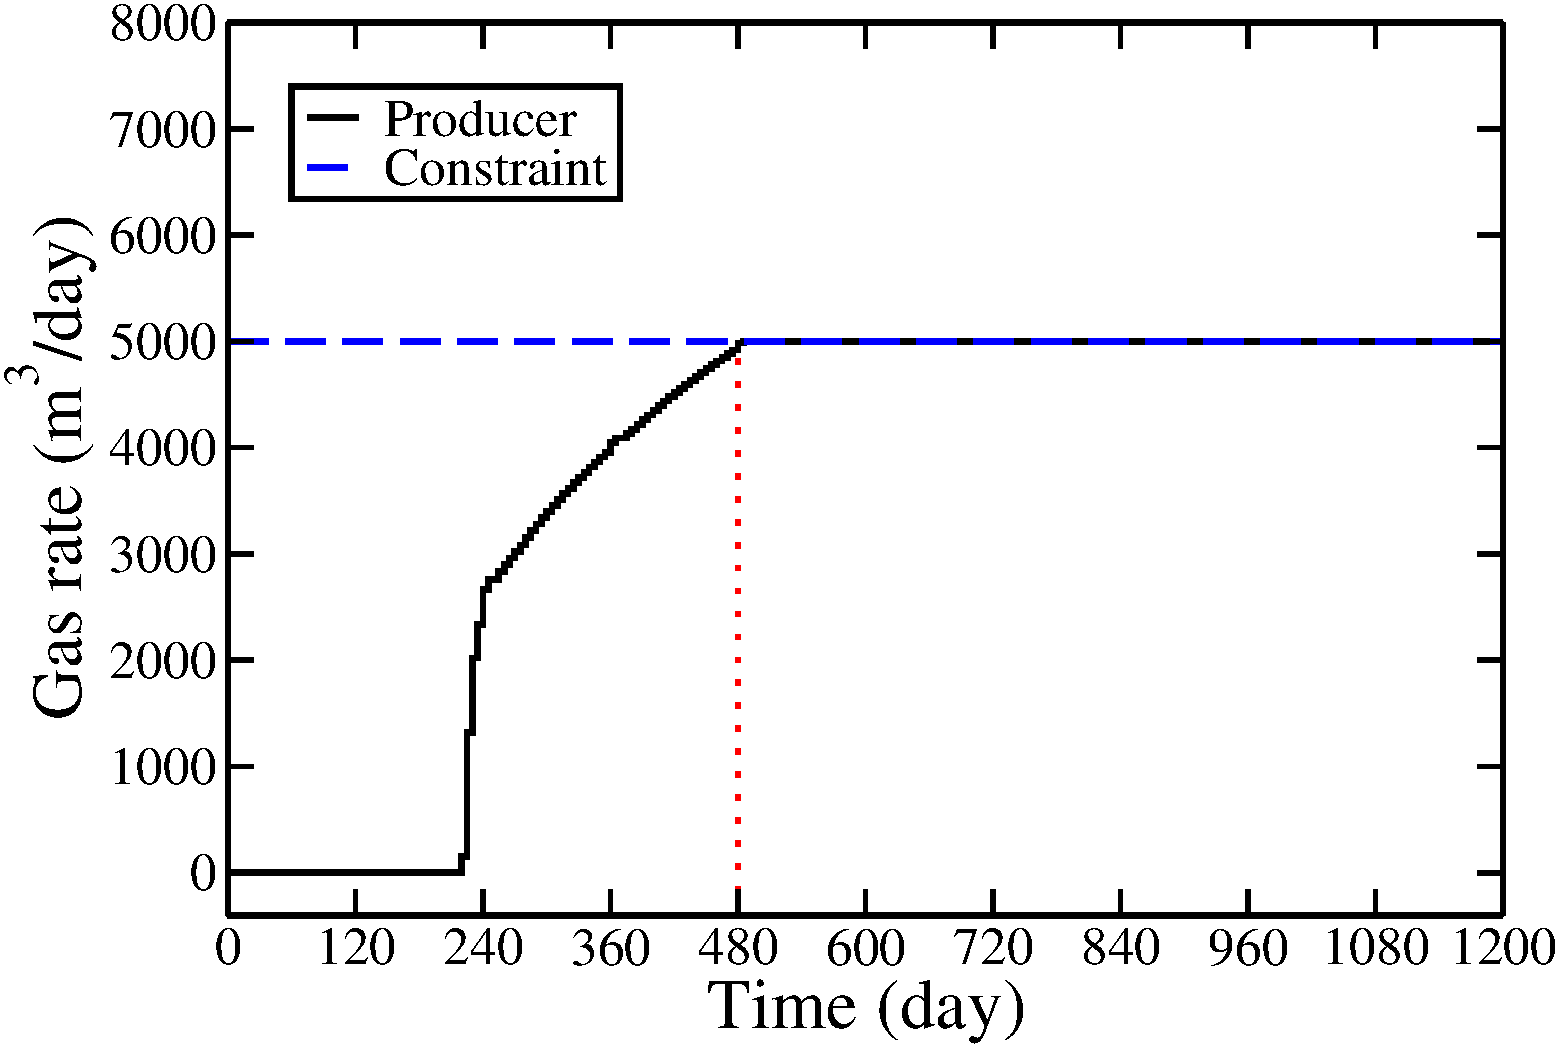
\includegraphics[height=2.7cm]{figures/SimpleRate_rate_gas.pdf} \\
  \end{tabular}
\end{center}
     \caption{Schematic illustrating heuristic constraint handling. Top: Constant BHP and resulting gas rate. Bottom: BHP and gas rate satisfying constraint.}
\label{fig:BHPvsRateControl}
\end{figure}


Although it is clearly approximate, this heuristic constraint handling approach
has some potential advantages over the formal method described in
Section~\ref{sec:constr-opt}. For example, the heuristic treatment allows the
simulator to switch controls at any time step in the simulation, while the
formal approach only allows controls to switch at a relatively small number of
control steps (by way of comparison, in a typical problem we may have
  $O(10^2-10^3)$ time steps but only $O(10)$ control steps). The heuristic
approach thus enables, in some sense, a more `fine-grained' response, and it can
be viewed as having many more `control' variables (though these variables are
  not optimized formally). Increasing the number of control steps to provide the
same granularity to the optimizer as in the forward problem (i.e., setting the
  control step size to equal the time step size) should theoretically result in
better performance by the formal approach, though in practice the large
increase in the number of control variables would result in a more difficult optimization
problem, which could negatively impact the performance of the optimizer. In the examples
below, we will compare the performance of these two approaches for handling
nonlinear constraints.

We note finally that if rates are used as the control variables, then the rate
constraints enter the optimization problem as simple bound constraints, which
are easy to satisfy. In this case, however, the BHPs become nonlinear
constraints. Our heuristic treatment would then entail the switch from rate
control to BHP control if the BHP constraint would otherwise be violated. We did
not test the performance of our procedure using rates as the control variables,
but this should be considered in future work.




